\mainsection{2}{Repaso de Medicion}{8/19/2021}

El PIB es el valor de los bines y servicios finales producidos en un territorio en un periodo determinado. El PIB per capita es la medida más común del bienestar económico. 

\section{Medicion de un Economia}

\textbf{Logartimo y tasas de crecimiento}

Sea $y_{t}$ el PIB real en el periodo $t$, y $\Delta$ su tasa de crecimiento

\begin{align*}
    \Delta y_{t+1} &= \frac{y_{t+1} - y_{t}}{y_{t}} \\
    \Delta y_{t+1} &= \frac{y_{t+1}}{y_{t}} - 1  \\
    \ln{(1+ \Delta y_{t+1})}  &= \ln{y_{t+1}} - \ln{y_{t}}
\end{align*}

Note que $\ln{(1+x)}\approx x$ si $x$ es pequeño, entonces

\begin{equation}
     \Delta y_{t+1}  \approx \ln{y_{t+1}} - \ln{y_{t}}
\end{equation}

La aproximación viene de una aproximación de una Serie de Taylor; así cuando $x$ es menor a $0,1$ se considera una estimación satisfactoria.

\begin{definition}
Producto interno Bruto es el \textbf{valor de mercado} de todos los vienes y servicios producidos domésticamente en una economía, en un periodo específico.
\end{definition}

Existen tres enfoques para medir el PIB, siendo \textbf{Enfoque de producto:} Al sumar el valor agregado de todas las industrias de economia. Luego el \textbf{enfoque de gasto:} Al sumar los gastos en bienes y servicios de todo los agentes. Por último \textbf{Enfoque del Ingreso:} Al sumar todos los ingresos generados en el proceso productivo.

\begin{definition}
\textbf{Valor Agregado:} es el valor de sus productos menos el valor de los insumos de consumo intermedio que usa una empresa para producir esos productos.
\end{definition}

\begin{definition}
\textbf{Consumo Intermedio:} Son los productos utilizados como insumos por las unidades productivos en su proceso de producción.
\end{definition}

\textbf{Las Cantidades nominales y reales pueden diferir}

\begin{definition}
\textbf{Valor Nominal: }denota el valor de mercado de una cantidad de producto, valorado a los precios definidos al momento de producción.
\end{definition}

\begin{definition}
\textbf{Valor Real: } denota el valor de mercado de una cantidad de producto, valorado a un conjunto de precios fijo
\end{definition}

\subsection{Inflación}

\begin{definition}
\textbf{Inflación} es el aumento sostenido y generalizado del nivel de precios.
Asi la tasa de inflación es el aumento porcentual del nivel de precios.
\end{definition}

Tome $P_{t}$ como una medida del nivel de precios:

\begin{equation}
   Inflacion = \frac{P_{t}-P_{t-1}}{P_{t-1}} \times 100
\end{equation}
\myequations{Inflacion}

\textbf{El deflactor del PIB} es la medida del nivel de precios defina como

\begin{equation}
    Deflactor = \frac{PIB Nominal}{PIB Real} \times 100
\end{equation}
\myequations{Deflactor del PIB}

El deflactor se llama así porque “desinfla” (remueve los efectos del cambio en el nivel de precios) el PIB y otras variables económicas

\textbf{Índice de Precios de Consumidor}, El IPC es otra medida ampliamente utilizada para medir el nivel de precios, incluye bienes y servicios comprados por los \textbf{consumidores}. En Costa Rica es el \textbf{INEC} quien se encarga de elaborarlo. 

El indice se calcula de forma mensual con la informacion de los precios de los articulos. Calcula el precio de la canasta de la forma:
\begin{equation}
    IPC = \frac{\textup{Costo de la canasta en precios corrientes}}{\textup{Costo de la canasta a precios baces}} \times 100
\end{equation}
\myequations{Formula del IPC}

Para esto podemos entablar una lista de la diferencias entre usar el IPC y deflator del PIB, asi entonces:

\begin{table}[H]
\centering
\begin{tabular}{l|l}
IPC                               & Deflactor                            \\ \hline
Excluye precios de bines de Capital. & \begin{tabular}[c]{@{}l@{}}Incluye precios de bienes de \\ capital producidos domesticamente.\end{tabular} \\
Incluye bienes Importados.         & Excluye bienes de consumo importados. \\
Basado en Canasta fija: Laspeyres. & Basado en una canasta variable.      
\end{tabular}
\end{table}

\begin{figure}[H]
    \centering
    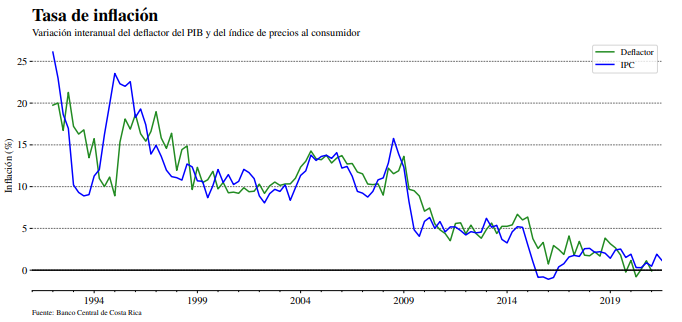
\includegraphics[scale=0.5]{Images/inflacion.png}
    \caption{Comparación Inflación IPC y Deflactor del PIB}
    \label{fig:my_label}
\end{figure}

\textbf{Problemas con la medición del Precios}

Al usar una canasta fija no puedo reflejaran la sustitución que hacen los hogares hacia los bienes que se abaratan. Así también \textbf{no miden todos los cambios en la calidad} ni tampoco la introducción de nuevos bienes en una economía.

\subsection{Índices de Precios: Laspeyres}

Un índice de precios de Laspeyres valora una canasta de productos a precios de año base:

\begin{equation}
    Lp(t) = \frac{\sum_{i=1}^{I}p_{i}(t)q_{i}(b)}{\sum_{j=1}^{I}p_{j}(b)q_{j}(b)}
\end{equation}

\myequations{Indice de Precios Laspeyres}

Donde $i$ denota la cantidad de los artículos, $b$ es el periodo base y $p_{i}(t)$ es el precio relativo del articulo $i$, de forma análoga $q_{i}(t)$ es la cantidad del articulo $i$.

Las Canastas deben actualizarse periódicamente debe mantener validez, las canastas fijas se vuelven menos representativas entre mas lejos estén del año base.

El índice encadenado se calcula cambio porcentual, se elige un periodo de referencia donde se normaliza el índice encadenado. Después se encadena toda la serie por medio de los cambios porcentuales del paso inicial. 

\begin{align}
    \tilde{Lp}(0)&= 1\\
    \tilde{Lp}(y) &= \prod^{t}_{\tau =1} \frac{\sum_{i=1}^{I_{\tau}}p_{i}(\tau)q_{i}(\tau-1)}{\sum_{j=1}^{I_{\tau}}p_{j}(\tau-1)q_{j}(\tau-1)}
\end{align}
\myequations{Indice de Laspeyres Encadenado}

Soluciona los problemas de obsolescencia de: Canasta de bienes base y el conjunto de pecios base. 

\textbf{Medidas subyacentes de inflacion}

No todo precio que cambie es inflacion:

\begin{itemize}
    \item Los precios relativos pueden cambiar por: Escasez o abundancia de los bienes y factores institucionales.
    \item La inflación es un proceso \textbf{generalizado y sostenido de aumento precios} debido fundamentalmente a presiones monetarias.
    \item Hay cambios que afectan al IPC o al deflactor que no son propios de la inflación.
\end{itemize}

Por ello utilizamos ciertas medidas, exclusión a priori de un conjunto de productos. Exclusión por volatilidad histórica de producto. Truncamiento asimétrico de la distribución del IPC. Reponderación de productos según volatilidad y persistencia.

\subsection{Ciclos Económicos: Descomposición de series de tiempo}

Las series de tiempo generalmente se separan en cuatro componentes:

\begin{equation}
    Y_{t}=T_{t}+C_{t} +S_{t} +\epsilon_{t}
\end{equation}

\myequations{Composición de series del tiempo}

La tendencia $T$ refleja el comportamiebnto de la serie a largo plazo.

El ciclo $C$ refleja comportamientos que son de naturaleza \textbf{recurrente, aunque no exactamente periódicos}, cuya periodicidad es mayor a un año.

El componente estacional $S$ recoge oscilaciones regulares.

Y un componente estocástico $\epsilon$ que no presentan periodicidad.

\begin{definition}
Los \textbf{ciclos económicos} reflejan desviaciones con respecto a la tendencia de largo plazo. La duración de los ciclos es bastante irregular, es definir el momento de los cambios en el ciclo. La predecibilidad de un ciclo yace en \textbf{comovimiento} muchas variables macroeconómicas se mueven de manera bastante predecible.
\end{definition}

Ajuste estacional, el componente estacional $S_{t}$ recoge las oscilaciones regulares en los distintos periodos. Para eliminar el efecto de estos factores y poder concentrarse en los ciclos y la tendencia usualmente. 